\documentclass[journal,10pt,twocolumn]{article}
\usepackage{graphicx}
\usepackage[margin=0.5in]{geometry}
\usepackage[cmex10]{amsmath}
\usepackage{array}
\usepackage{booktabs}
\usepackage{mathtools}
\title{\textbf{Conic section Assignment}}
\author{Mohamed Hamdan}
\date{September 2022}


\providecommand{\norm}[1]{\left\lVert#1\right\rVert}
\providecommand{\abs}[1]{\left\vert#1\right\vert}
\let\vec\mathbf
\newcommand{\myvec}[1]{\ensuremath{\begin{pmatrix}#1\end{pmatrix}}}
\newcommand{\mydet}[1]{\ensuremath{\begin{vmatrix}#1\end{vmatrix}}}
\providecommand{\brak}[1]{\ensuremath{\left(#1\right)}}

\begin{document}

\maketitle
\paragraph{\textit{Problem Statement} - Find the area of the triangle formed by the lines joining the vertex of the parabola $x^2 = 12y$ to the ends of its latus rectum}

\section*{\large Solution}

\begin{figure}[h]
\centering
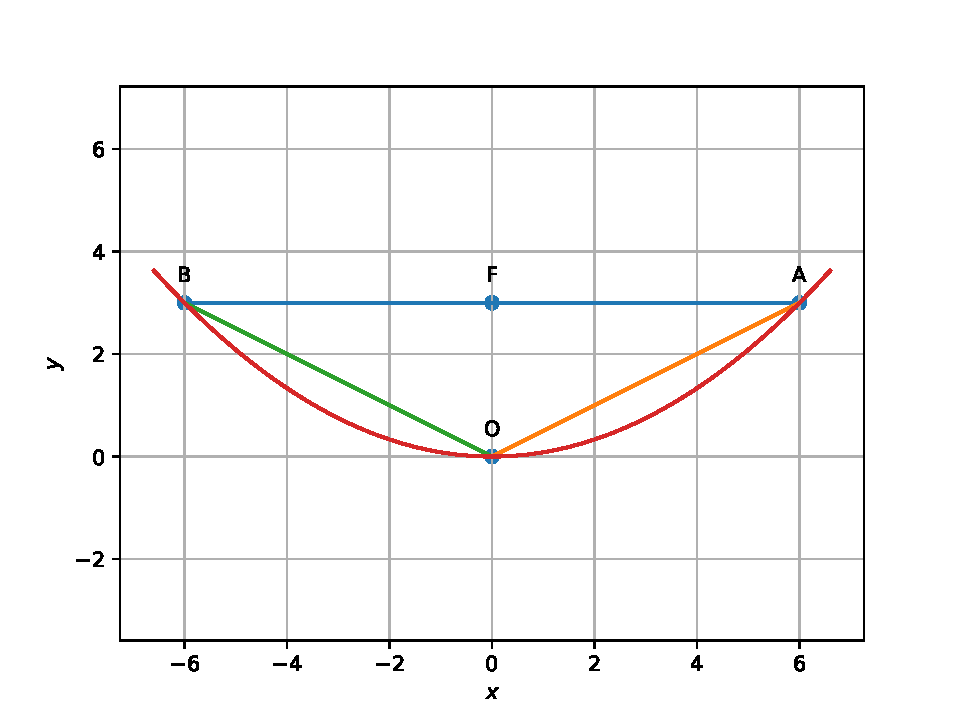
\includegraphics[width=1\columnwidth]{figs/fig1.pdf}
\caption{Triangle formed by vertex and ends of latus rectum of parabola $x^2 = 12y$}
\label{fig:parabola}
\end{figure}

The given equation of parabola $x^2 = 12y$ can be written in the general quadratic form as
\begin{align}
    \label{eq:conic_quad_form}
    \vec{x}^{\top}\vec{V}\vec{x}+2\vec{u}^{\top}\vec{x}+f=0
    \end{align}
where
\begin{align}
	\label{eq:V_matrix}
	\vec{V} &= \myvec{1 & 0\\0 & 0},
	\\
	\label{eq:u_vector}
	\vec{u} &= \myvec{0\\-6},
	\\
	\label{eq:f_value}
	f &= 0
	%\\
\end{align}

The parabola in (\ref{eq:conic_quad_form}) can be expressed in standard form (center/vertex at origin, major-axis - $x$ axis) as
\begin{align}
	\label{eq:conic_simp_parab}
	\vec{y}^{\top}\vec{D}\vec{y} &=  -2\eta\vec{e}_1^{\top}\vec{y}   & \abs{V} &= 0
	\end{align}
 where
\begin{align}
	\label{eq:conic_affine}
	\vec{x} = \vec{P}\vec{y}+\vec{c} \quad \text{(Affine Transformation)}
\end{align}
\begin{align}
	\label{eq:conic_parmas_eig_def}
	\vec{P}^{\top}\vec{V}\vec{P} &= \vec{D}. \quad \text{(Eigenvalue Decomposition)}
	\\
	\label{eq:eigevalV}
	\vec{D} &= \myvec{\lambda_1 & 0\\ 0 & \lambda_2}, 
	\\
	\vec{P} &= \myvec{\vec{p}_1 & \vec{p}_2}, \quad \vec{P}^{\top}=\vec{P}^{-1},
	\label{eq:eigevecP}
	\\
	\label{eq:eta}
	\eta &=\vec{u}^{\top}\vec{p}_1
	\\
	\vec{e}_1 &=\myvec{1 \\ 0}
	\end{align}

To find $\vec{c}$ which is the center of the parabola in (\ref{eq:conic_quad_form}), substitute (\ref{eq:conic_affine}) in (\ref{eq:conic_quad_form})
\begin{multline}
\brak{\vec{P}\vec{y}+\vec{c}}^T\vec{V}\brak{\vec{P}\vec{y}+\vec{c}}+2\vec{u}^T\brak{\vec{P}\vec{y}+\vec{c}} + f = 0, 
\end{multline}
yielding 
\begin{multline}
\vec{y}^T\vec{P}^T\vec{V}\vec{P}\vec{y}+2\brak{\vec{V}\vec{c}+\vec{u}}^T\vec{P}\vec{y} +  \vec{c}^T\vec{V}\vec{c} 
\\
+2\vec{u}^T\vec{c} + f= 0
\label{eq:conic_simp_one}
\end{multline}
%
From \eqref{eq:conic_simp_one} and \eqref{eq:conic_parmas_eig_def},
\begin{multline}
\vec{y}^T\vec{D}\vec{y}+2\brak{\vec{V}\vec{c}+\vec{u}}^T\vec{P}\vec{y} +  \vec{c}^T\brak{\vec{V}\vec{c} + \vec{u}}
\\
+ \vec{u}^T\vec{c} + f= 0
\label{eq:conic_simp}
\end{multline}
For a parabola $\abs{\vec{V}} = 0, \lambda_1 = 0$ and
\begin{align}
\vec{V}\vec{p}_1 = 0, 
\vec{V}\vec{p}_2 = \lambda_2\vec{p}_2.
\label{eq:conic_parab_eig_prop} 
\end{align}
where $\vec{p}_1,\vec{p}_2$ are the eigenvectors of $\vec{V}$ such that  \eqref{eq:conic_parmas_eig_def}
%
\begin{align}
\vec{P} = \myvec{\vec{p}_1 & \vec{p}_2},
\label{eq:eig_matrix}
\end{align}
Substituting \eqref{eq:eig_matrix}
in \eqref{eq:conic_simp},
\begin{multline}
	\vec{y}^T\vec{D}\vec{y}+2\brak{\vec{c}^T\vec{V}+\vec{u}^T}\myvec{\vec{p}_1 & \vec{p}_2}\vec{y}
\\
+  \vec{c}^T\brak{\vec{V}\vec{c} + \vec{u}}+ \vec{u}^T\vec{c} + f= 0
\\
\implies \vec{y}^T\vec{D}\vec{y}
\\
+2\myvec{\brak{\vec{c}^T\vec{V}+\vec{u}^T}\vec{p}_1  \brak{\vec{c}^T\vec{V}+\vec{u}^T}\vec{p}_2}\vec{y}
\\
+  \vec{c}^T\brak{\vec{V}\vec{c} + \vec{u}}+ \vec{u}^T\vec{c} + f= 0
\\
\implies \vec{y}^T\vec{D}\vec{y}
\\
+2\myvec{\vec{u}^T\vec{p}_1 & \brak{\lambda_2\vec{c}^T+\vec{u}^T}\vec{p}_2}\vec{y}
\\
+  \vec{c}^T\brak{\vec{V}\vec{c} + \vec{u}}+ \vec{u}^T\vec{c} + f= 0
\text{ from } \eqref{eq:conic_parab_eig_prop}     \nonumber \\
\\
\implies \lambda_2y_2^2+2\brak{\vec{u}^T\vec{p}_1}y_1+  2y_2\brak{\lambda_2\vec{c}+\vec{u}}^T\vec{p}_2
\\
+  \vec{c}^T\brak{\vec{V}\vec{c} + \vec{u}}+ \vec{u}^T\vec{c} + f= 0
\label{eq:conic_parab_foc_len_temp} 
\end{multline}
which is the equation of a parabola. 
Thus, \eqref{eq:conic_parab_foc_len_temp} 
can be expressed as \eqref{eq:conic_simp_parab} by choosing
\begin{align}
%\label{eq:eta}
\eta = \vec{u}^T\vec{p}_1
\end{align}
and $\vec{c}$ in \eqref{eq:conic_simp} such that
\begin{align}
\label{eq:conic_parab_one}
\vec{P}^{T}\brak{\vec{V}\vec{c}+\vec{u}} &= \eta\myvec{1\\0}
\\
\vec{c}^T\brak{\vec{V}\vec{c} + \vec{u}}+ \vec{u}^T\vec{c} + f&= 0
\label{eq:conic_parab_two}
\end{align}
Multiplying \eqref{eq:conic_parab_one} by $\vec{P}$ yields
\begin{align}
\label{eq:conic_parab_one_eig}
\brak{\vec{V}\vec{c}+\vec{u}} &= \eta\vec{p}_1,
\end{align}
which, upon substituting in \eqref{eq:conic_parab_two}
results in 
\begin{align}
\eta\vec{c}^T\vec{p}_1 + \vec{u}^T\vec{c} + f&= 0
\label{eq:conic_parab_two_eig}
\end{align}
\eqref{eq:conic_parab_one_eig} and \eqref{eq:conic_parab_two_eig} can be clubbed together to obtain \eqref{eq:conic_parab_c}.
\begin{align}
    \myvec{ \vec{u}^{\top}+\eta\vec{p}_1^{\top} \\ \vec{V}}\vec{c} &= \myvec{-f \\ \eta\vec{p}_1-\vec{u}}  &\abs{V} &= 0
    \label{eq:conic_parab_c}
    \end{align}
Substituting appropriate values from \eqref{eq:V_matrix}, \eqref{eq:u_vector}, \eqref{eq:f_value}, \eqref{eq:eigevecP}, and \eqref{eq:eta} into \eqref{eq:conic_parab_c}, the below matrix equation is obtained
\begin{align}
	\label{eq:vertex_system}
	\myvec{0&-12\\1& 0\\0& 0}\vec{c} = \myvec{0 \\0 \\0}\\
\end{align}
The augmented matrix for \eqref{eq:vertex_system} can be expressed as
\begin{align}
	\label{eq:vertex_solv1}
	\myvec{0&-12&\vrule&0\\1&0&\vrule&0\\0&0&\vrule&0}\\ 	
	\label{eq:vertex_solv2}
	\xleftrightarrow[]{R_1 \leftrightarrow R_2}\myvec{1&0&\vrule&0\\0&-12&\vrule&0\\0&0&\vrule&0}\\
	\label{eq:vertex_solv3}
	\xleftrightarrow[]{-\frac{R_2}{12} \leftarrow R_2}\myvec{1&0&\vrule&0\\0&1&\vrule&0\\0&0&\vrule&0}\\
	\label{eq:vertex_solv4}
	\implies\vec{c} = \myvec{0\\0}
\end{align}
\eqref{eq:vertex_system}
The latus rectum of a conic section is the chord that passes through the focus, is perpendicular to the major axis and has both endpoints on the curve.\\\\For the parabola given by \eqref{eq:conic_simp_parab}, the focus and the foot of the directrix lie on the x-axis at  $l\vec{e}_1$ and $-l\vec{e}_1$ respectively where $\abs{l}$ is the focal length of the parabola. This is due to the fact that the vertex $(0,0)$ must be equidistant from the focus and the directrix.\\\\An end-point of the latus rectum is located at a distance of $2\abs{l}$ from the directrix. Since a point on the parabola is equidistant from the directrix and the focus and the latus rectum passes through the focus, an endpoint of the latus rectum can be assumed as
\begin{equation}
\begin{aligned}
	\vec{t}_1 &= l\myvec{1 \\ 2}\\
	\vec{t}_2 &= l\myvec{1 \\ -2}
\end{aligned}
	\label{eq:latus_endpoint}
\end{equation}
Substituting any point of \eqref{eq:latus_endpoint} in \eqref{eq:conic_simp_parab} and solving for $l$,
\begin{align}
	l &= -\frac{\eta}{2\lambda_2}
	\label{eq:focal_point}
\end{align}
Substituting \eqref{eq:focal_point} back in \eqref{eq:latus_endpoint}, the endpoints of the latus rectum is found.

The area of the traingle AOB is given by
\begin{align}
	ar(AOB) &= \frac{1}{2}AB.OF\\
	\label{eq:triangle}
\end{align}
where
\begin{align}
	\label{eq:base}
	AB &= \abs{\vec{e}_2^{\top}(\vec{t}_1-\vec{t}_2)}\\
	\label{eq:height}
	OF &= \abs{l}
\end{align}
First substitute \eqref{eq:latus_endpoint} in \eqref{eq:base}. Then substitute \eqref{eq:focal_point} in \eqref{eq:base} and \eqref{eq:height}. Finally, substituting \eqref{eq:base} and \eqref{eq:height} in \eqref{eq:triangle}, we get
\begin{align}
	ar(AOB) = \frac{\eta^2}{2\lambda_2^2}
\end{align}

\section*{\large Construction}
The input parameters are $\vec{V}$ from \eqref{eq:V_matrix}, $\vec{u}$ from \eqref{eq:u_vector} and $f$ from \eqref{eq:f_value}\\\\
{
\setlength\extrarowheight{5pt}
\begin{tabular}{|c|c|c|}
	\hline
	\textbf{Symbol}&\textbf{Value}&\textbf{Description}\\
	\hline
	$\vec{P}$&\myvec{0&1\\1&0}&eigenvectors of $\vec{V}$\\[5pt]
	\hline
	$\vec{c}$&$\myvec{0\\0}$&center of parabola\\
	\hline
	$\eta$&$\vec{u}^{\top}\vec{p}_1$&from \eqref{eq:eta}\\[5pt]
	\hline
	$\lambda_2$&$\vec{e}_2^{\top}D\vec{e}_2$&from \eqref{eq:eigevalV}\\[5pt]
	\hline
	$l$&$-\frac{\eta}{2\lambda_2}$&x coordinate of focus\\[5pt]
	\hline
	$(\vec{A},\vec{B})$&$\vec{P}\myvec{l&l\\2l&-2l} + \vec{c}$&endpoints of latus rectum\\[5pt]
	\hline
	$ar(AOB)$&$\frac{\eta^2}{2\lambda_2^2} = $18&ar(AOB) = 18 sq units\\[5pt]
	\hline
\end{tabular}
}

\end{document}
